\documentclass[a4paper]{article}
\author{
\includegraphics[width=0.2\textwidth]{images/logo_fundacio.png}
}
\title{\textbf{Manual d'usuari \emph{fiberfy-nt}}}

\usepackage{xcolor}
\usepackage{float}
\usepackage{graphicx}
\usepackage{titlesec}
\usepackage{subcaption}
\usepackage{setspace}
\usepackage{hyperref}
\usepackage[utf8]{inputenc}
\usepackage[catalan]{babel}

\definecolor{mygreen}{rgb}{0,0.6,0}
\definecolor{mygray}{rgb}{0.5,0.5,0.5}
\definecolor{mymauve}{rgb}{0.58,0,0.82}

\date{\today}
\titleformat{\section}
{\normalfont\fontsize{16}{18}\bfseries}{\thesection}{1em}{}

\titlespacing*{\section}
{0pt}{5.5ex plus 1ex minus .2ex}{4.3ex plus .2ex}
\titlespacing*{\subsection}
{0pt}{5.5ex plus 1ex minus .2ex}{4.3ex plus .2ex}
\titlespacing*{\subsubsection}
{0pt}{5.5ex plus 1ex minus .2ex}{1.3ex plus .2ex}

\addtolength{\oddsidemargin}{-.875in}
\addtolength{\evensidemargin}{-.875in}
\addtolength{\textwidth}{1.75in}
\addtolength{\topmargin}{-.875in}
\addtolength{\textheight}{1.75in}

\begin{document}
	\maketitle
	\newpage
	
	\begin{center}
		\begin{tabular}{| p{1.89cm} | p{2.21cm} | p{8.42cm} |} \hline
			\multicolumn{3}{|c|}{\large{\textbf{Historial de versions}}} \\ \hline
			\textbf{Versió} & \textbf{Data} & \textbf{Canvis} \\ \hline
			prototip & 10/08/2017 & Primera edició del document. Versió antiga del fiberfy \\ \hline
			18.10 & 11/10/2018 & Primera versió estable de l'aplicació. Canvis rellevants:
			\begin{itemize}
				\item El frontend canvia el nom a fiberfy-nt
				\item Es refà per complet l'aplicació només mantenint els mapes
				\item S'incorpora un importador de projectes
				\item S'incorpora un nou tipus de localització: No Definit
				\item Es demana confirmació al eliminar entitats
				\item S'incorpora un buscador de projectes
			\end{itemize} \\ \hline
		\end{tabular}
	\end{center}
	\newpage
	\tableofcontents
	\newpage
	\onehalfspacing
	
	\section{Introducció}
	L'eina de desplegaments de fibra òptica \emph{fiberfy-nt} ha estat creada per facilitar la confecció de projectes als diferents operadors de la xarxa \textbf{Guifi.net}.
	Aquest document és manual d'usuari per ensenyar les característiques de l'aplicació i explicar-ne el seu funcionament. 
	
	\section{Accés al portal}
	L'aplicació \emph{fiberfy-nt} és un servei web accessible des de qualsevol dipositiu amb un navegador compatible amb \textbf{JavaScript}. La seva direcció és: \url{https://fiberfy.guifi.net/}
	
	\begin{figure}[H]
		\centering
		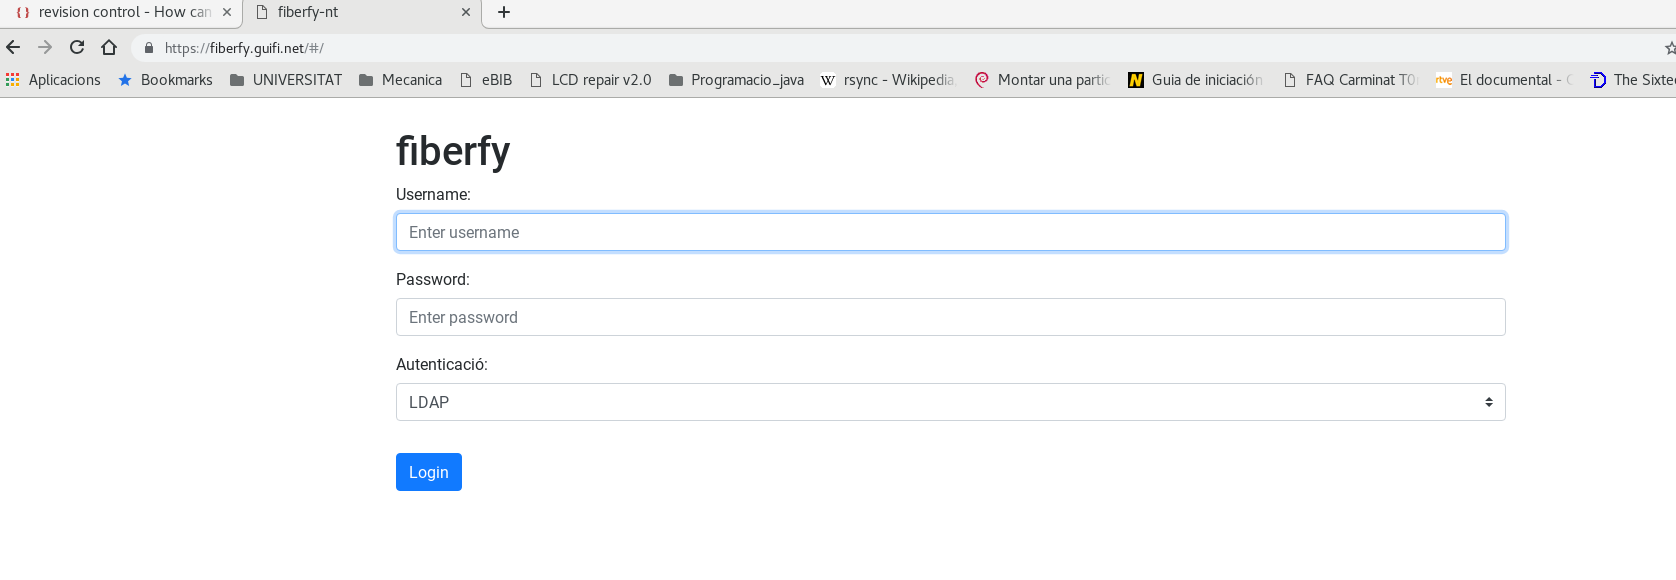
\includegraphics[width=0.7\textwidth]{images/login_screen.png}
		\caption{Pantalla de login \emph{fiberfy-nt}}
	\end{figure}

	Els paràmetres d'accés vindran subministrats per la fundació. Actualment es pot autenticar usuaris mitjançant l'\textbf{LDAP} del \textbf{GLIR}, per tant l'usuari podrà usar el mateix usuari pels diferents serveis que s'ofereixen. Un cop l'usuari s'ha autenticat li apareixerà un mapa de Catalunya.
	
	\begin{figure}[H]
		\centering
		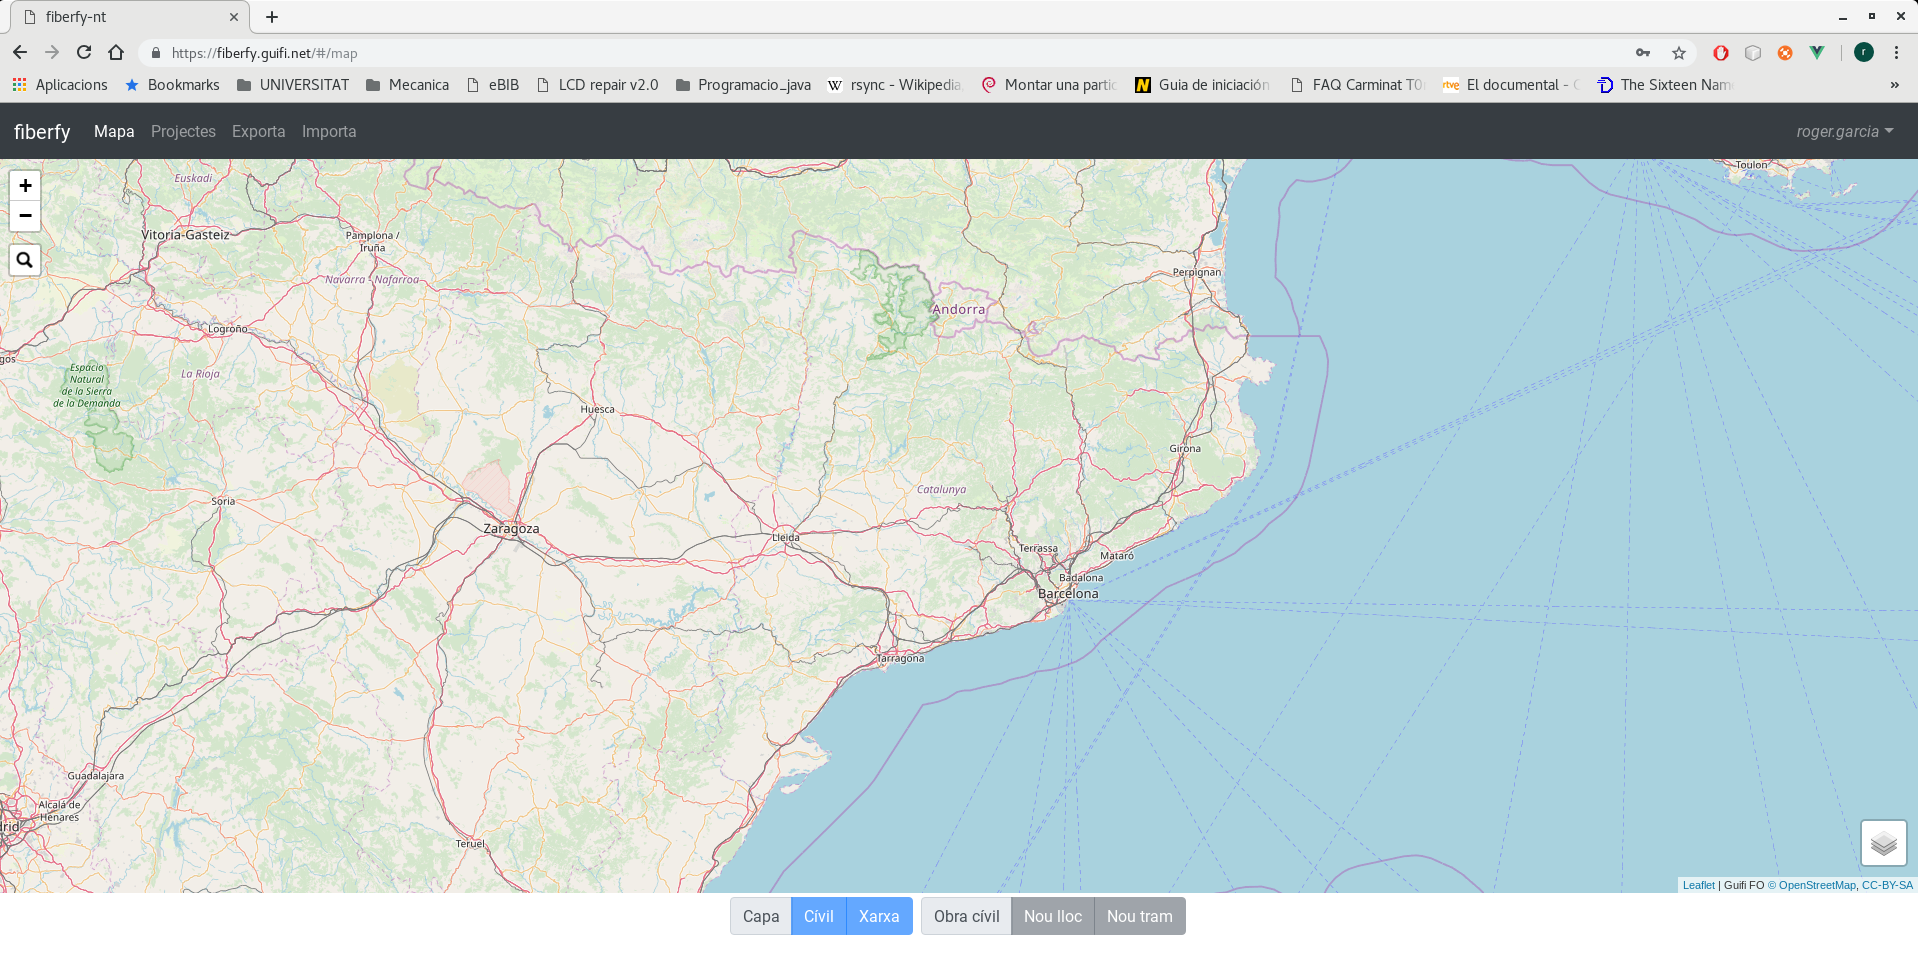
\includegraphics[width=0.7\textwidth]{images/map_screen.png}
		\caption{Mapa d'inici \emph{fiberfy-nt}}
	\end{figure}

	\section{Funcionament del mapa}
	El mapa ens permet treballar amb diferents capes. Hi ha dos tipus de capes:
	\begin{itemize}
		\item Capes base: Aquestes són les capes bàsiques que ens gràfiquen l'esquelet del mapa; només s'en pot seleccionar una a la vegada. A dia d'avui tenim la capa gratuïta d'\textbf{OpenStreetMap} i diverses capes de \textbf{Google}.
		\item Capes auxiliars: Aquestes són capes que es mostren a sobre de la capa base i ens aporten informació extra. Actualment disposem de 4 capes de Guifi.net (nodes, enllaços, localitzacions (fibra), trams (fibra).
	\end{itemize}
	Per interactuar amb les diferents capes del mapa situarem el punter sobre un pictograma situat al extrem inferior dret com podem veure a la figura \ref{fig:pictogram-layer}:
	
	\begin{figure}[H]
		\centering
		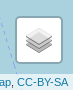
\includegraphics{images/pictogram_layer.png}
		\caption{Pictograma gestió de capes}
		\label{fig:pictogram-layer}
	\end{figure}

	A la figura \ref{fig:layer-manager} podem veure el gestor de capes del mapa.
	\begin{figure}[H]
		\centering
		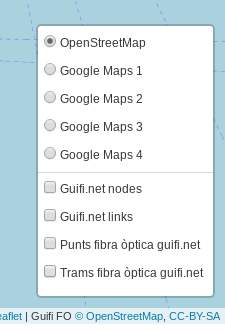
\includegraphics{images/layer_manager.png}
		\caption{Menú de gestió de capes}
		\label{fig:layer-manager}
	\end{figure}
	
	\section{Gestió de projectes}
	Per tal de crear projectes haurem d'accedir al menú situat a la capçalera de la pàgina i accedirem a la pestanya de projectes.
	
	\begin{figure}[H]
		\centering
		
\includegraphics{images/topbar_menu_1.png}
		\caption{Menú superior \emph{fiberfy-nt}}
	\end{figure}
	Al formulari de projectes ens apareixerà primer una petita targeta amb la informació del projecte seleccionat que ens permetrà modificar les seves característiques:
	\begin{itemize}
		\item \textbf{Guardar Posició}: Aquest botó ens guarda la posició del mapa actual al projecte. Així quan tornem a utilitzar l'aplicació ens mantindrà aquesta posició i no haurem de navegar pel mapa buscant-lo.
		\item \textbf{Editar}: Aquest botó ens porta a un formulari on podrem modificar els atributs del projecte
	\end{itemize}
	Ens apareixerà un buscador de projectes i a la part inferior es mostraran els resultats obtinguts. Per defecte es mostren tots els projectes; si l'usuari desitja mostrar tots els projectes després d'haver fet una búsqueda haurà de borrar el text i tornar a prémer \textbf{Buscar}.
	Els projectes de cada usuari seran visibles per tots els usuaris i només podran ser modificats per ell mateix. Per tal de treballar sobre qualsevol projecte aquest s'haurà d'activar prement el botó \textbf{Activar} situat a la barra de botons de la dreta.
	
	\begin{figure}[H]
		\centering
		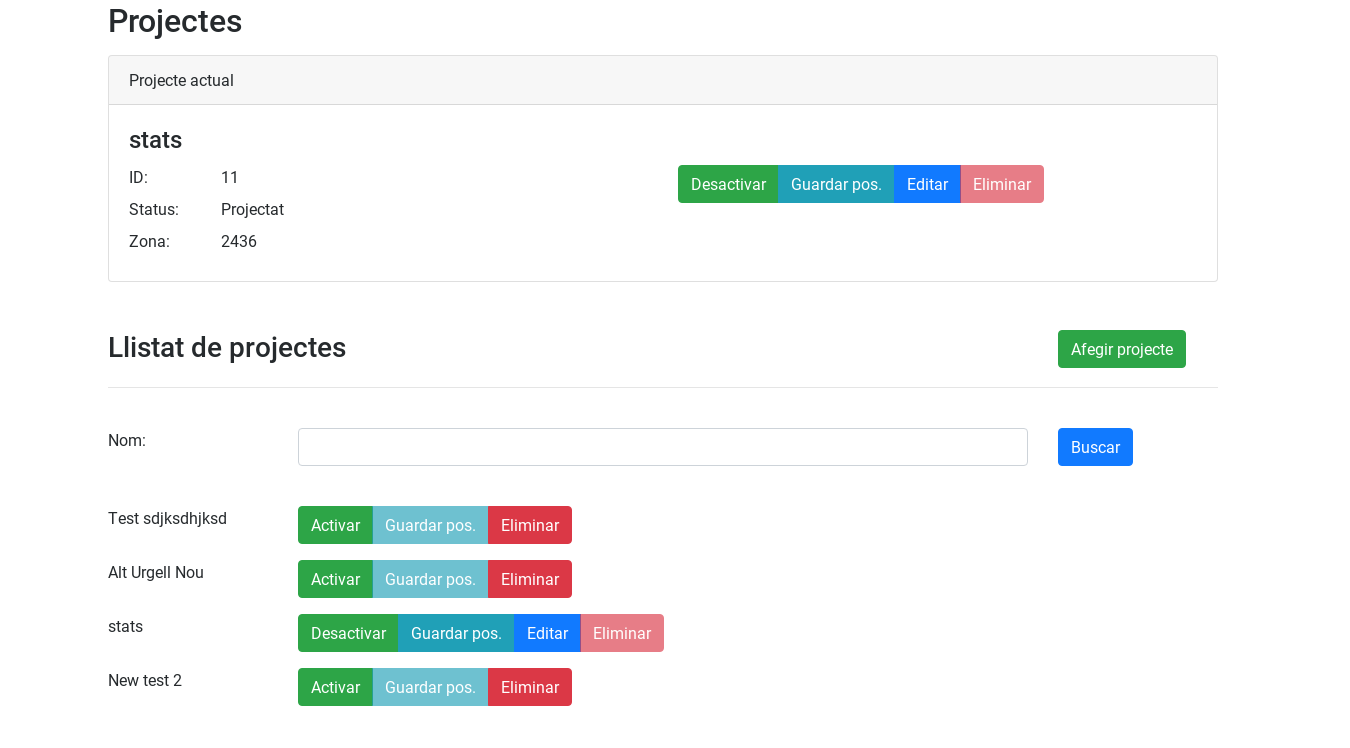
\includegraphics[width=0.8\textwidth]{images/projects_form.png}
		\caption{Formulari de projectes \emph{fiberfy-nt}}
	\end{figure}

	Per tal de crear nous projectes haurem de prémer el botó verd \textbf{Nou projecte} situat a la part superior dreta del Llistat de projectes.
	
	\subsection{Edició}
	Per tal d'editar projectes l'usuari haurà de prémer el botó blau \textbf{Editar} i serà conduït a un formulari com el que podem veure a la següent figura:
	
	\begin{figure}[H]
		\centering
		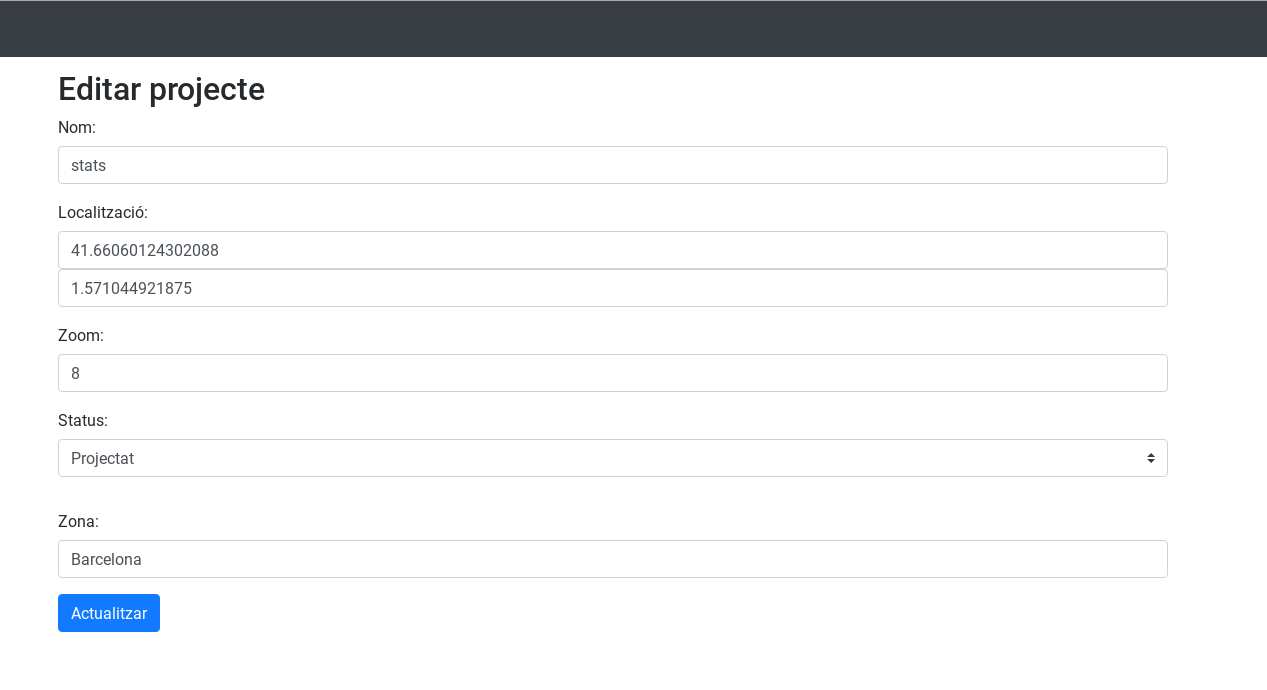
\includegraphics[width=0.8\textwidth]{images/project_edit_form.png}
		\caption{Formulari de projectes \emph{fiberfy-nt}}
	\end{figure}

	Aquí l'usuari podrà modificar aspectes com el nom del projecte, el punt de referència del mapa (Localització + zoom), status (el mateix que hi ha a la web de Guifi.net) i finalment la zona per defecte. La zona ve donada per la base de dades de Guifi.net (la mateixa que la web), l'usuari la pot seleccionar d'un desplegable a mesura que va escrivint.
	
	\section{Obra civil}
	\subsection{Gestió de sites}
	Els \emph{sites} dins de l'aplicació simbolitzen els punts físics d'obra civil on s'ubicaran les caixes i sistemes de telecomunicacions. Contenen unes coordenades i atribut físic que ens indica el tipus d'element. També permeten afegir comentaris i modificar-ne el nom.
	
	\subsubsection{Creació}
	Sobre el mapa inicial podem crear diferents \emph{sites} on s'ubicaran els equips de fibra òptica. Per tal de crear nous \emph{sites} hem de seleccionar la pestanya \emph{Crea Lloc} del menú superior. Aleshores hem d'anar marcant amb el botó esquerra del ratolí els punts on hi volem col·locar un nou \emph{site}. Per sortir del menú de creació de nous \emph{sites} podem clicar a qualsevol \emph{site} existent.
	
	\begin{figure}[H]
		\centering
		%\includegraphics[width=0.7\textwidth]{menu_lloc_fiberfy.png}
		\caption{Menú de creació \emph{sites}}
	\end{figure}

	Els \emph{sites} creats se simbolitzaran utilitzant uns quadrats de color vermell.
	
	\begin{figure}[H]
		\centering
		%\includegraphics[width=0.7\textwidth]{sites_fiberfy.png}
		\caption{Mapa amb \emph{sites}}
	\end{figure}

	\subsubsection{Edició}
	Per editar un \emph{site} des del menú d'\emph{Obra Civil} hem de clicar sobre el \emph{site} del mapa que volem modificar. Aleshores s'ens projectarà un formulari amb tots els atributs rellevants pel \emph{site}. Els atributs modificables són: les coordenades, el nom, el tipus de \emph{site} i la possible observació(comentari).
	
	\begin{figure}[H]
		\centering
		%\includegraphics[width=0.7\textwidth]{lloc_form_fiberfy.png}
		\caption{Formulari de \emph{sites}}
	\end{figure}

	Si hem realitzat qualsevol modificació que volem guardar abans de tornar al mapa haurem de clicar el botó \emph{Update}.
	
	Si volem eliminar el \emph{site} haurem de clicar el botó \emph{Delete} i automàticament serem redirigits al mapa.
	
	\subsection{Gestió de trams}
	Els \emph{trams} dins de l'aplicació ens indicaran l'obra civil encarregada d'unir uns determinats \emph{sites}. Podrem definir com serà aquest \emph{tram} i escriure alguna anotació(observation).
	
	\subsubsection{Creació}
	Per tal de crear \emph{trams} haurem de seleccionar la pestanya \emph{Crea Tram} del menú superior. Un cop seleccionada la pestanya hem de clicar sobre el primer \emph{site} que volem unir i anar clicant sobre els següents \emph{sites} adjacents tot traçant una línia.
	
	\begin{figure}[H]
		\centering
		%\includegraphics[width=0.7\textwidth]{trams_fiberfy.png}
		\caption{Mapa amb \emph{trams}}
	\end{figure}
	
	Si volem unir diferents \emph{sites} amb un recorregut no recte, podem afegir punts al traçat marcant els punts de vèrtex sobre el mapa després d'haver marcat el primer \emph{site} i tancant el traçat al marcar el segon \emph{site}
	
	\begin{figure}[H]
		\centering
		%\includegraphics[width=0.7\textwidth]{trams_curve_fiberfy.png}
		\caption{Mapa amb \emph{trams} no rectes}
	\end{figure}

	Per sortir del menú de creació de nous \emph{trams} podem clicar a qualsevol \emph{tram} existent.
	
	\subsubsection{Edició}
	Per editar un \emph{tram} haurem de marcar la pestanya \emph{Crear Tram} com si volguéssim afegir nous trams i llavors haurem de clicar sobre el tram a modificar. Aleshores ens apareixerà un formulari amb tots els atributs que podem alterar.
	
	\begin{figure}[H]
		\centering
		%\includegraphics[width=0.7\textwidth]{tram_form_fiberfy.png}
		\caption{Formulari d'edició de \emph{trams}}
	\end{figure}

	Si hem fet alguna modificació i la volem guardar haurem de clicar el botó \emph{Update}.
	Si volem eliminar el tram haurem de clicar el botó \emph{Delete} i automàticament serem redirigits al mapa.
	\section{Cablejat}
	\subsection{Gestió de caixes}
	Les caixes són els elements de telecomunicacions per tal de connectar i distribuir les diferents fibres. Aquests elements són necessaris al inici i final d'una fibra.
	
	\subsubsection{Creació}
	Per tal de crear \emph{caixes} necessitarem haver definit prèviament un \emph{site} al punt on vulguem col·locar la \emph{caixa}. Un cop complert aquest requisit seleccionarem la pestanya \emph{Cablejat} i accedirem al menú de material de telecomunicació. Allà clicarem la pestanya de \emph{Crea Caixa} i marcarem el Site on anirà col·locada.
	
	\begin{figure}[H]
		\centering
		%\includegraphics[width=0.7\textwidth]{menu_caixa_buit_fiberfy.png}
		\caption{Menú de \emph{caixa} buit}
	\end{figure}

	Un cop ens aparegui el menú anterior haurem de triar el botó \emph{Nou} per tal de crear una nova \emph{caixa} en aquell \emph{site}. En un determinat \emph{site} s'hi poden col·locar tantes caixes com es desitgi.
	
	\subsubsection{Edició}
	Per tal de modificar els atributs d'una \emph{caixa} existent només caldrà clicar sobre la capsa en qüestió des del menú de cablejat de l'eina. Aleshores ens apareixarà el formulari de creació de \emph{caixes} amb les caixes existents en aquell \emph{site}. Per tal de modificar els atributs haurem de validar els canvis utilitzant el botó \emph{Update} del formulari. Per eliminar caixes haurem d'apretar el botó \emph{Delete}.
	
	Dins d'aquest formulari també podrem establir el tipus de capça que és i el nombre de fibres d'entrada i sortida que passaran per elles. Aquestes dades seran importants a l'hora de realitzar les fusions de fibres.
	
	\subsection{Gestió de fibra}
	Un cop les diferents caixes instal·lades ja podem fer passar les diferents fibres.
	
	\subsubsection{Creació}
	Per desplegar fibra entre dos punts del mapa necessitem que aquests estiguin units a través de diferents \emph{sites} i \emph{trams} i que continguin almenys una \emph{caixa}.
	Per començar hem de seleccionar el menú de \emph{Tirar Fibra} que trobarem al seleccionar la pestanya de \emph{Cablejat} que trobarem a la barra superior.
	
	\begin{figure}[H]
		\centering
		%\includegraphics[width=0.7\textwidth]{menu_cablejat_fiberfy.png}
		\caption{Menú de \emph{Cablejat} fiberfy}
	\end{figure}

	El següent pas serà clicar la pestanya de \emph{Tirar Fibra} del menú superior i marcar la caixa on anirà un dels extrems de la fibra. Aleshores anirem marcant un a un els \emph{sites} per on la fibra anira passant \footnote{Els extrems sempre han de contenir alguna \emph{caixa}}. Un cop acabada la trama de fibra per tal de validar-la haurem de marcar una segona vegada sobre l'últim \emph{site}.
	
	\begin{figure}[H]
		\centering
		%\includegraphics[width=0.7\textwidth]{fibres_fiberfy.png}
		\caption{Mapa amb \emph{fibres}}
	\end{figure}
	
	\subsubsection{Edició}
	
	Un cop tenim les \emph{fibres} creades i des del menú de \emph{Cablejat} podem clicar directament les fibres per tal de modificar-ne els atributs i afegir o treure línies de dins de la \emph{fibra}. Aquí també podrem seleccionar una configuració de \emph{fibra} des d'una \emph{Template} determinada. El formulari d'edició de fibres tindrà un format semblant al següent:
	
	\begin{figure}[H]
		\centering
		%\includegraphics[width=0.7\textwidth]{fibres_form_fiberfy.png}
		\caption{Formulari d'edició de \emph{fibres}}
	\end{figure}
	
	Per tal de guardar els canvis fets haurem de prémer el botó \emph{Update}. Si volem borrar la fibra haurem d'apretar el botó \emph{Delete}.
	
	\subsection{Gestió de fusions}
	Les fusions són les unions entre diferents fibres d'un cable fibra òptica. Per tal de poder realitzar fusions necessitem com a mínim un cable que contingui fibres tot-hi que el cas d'ús habitual és el d'unir diferents cables.
	
	\subsubsection{Creació i edició}
	Per tal de crear \emph{fusions} entre fibres hem d'accedir al menú de \emph{Cablejat} i clicar sobre la \emph{caixa} on volem practicar la \emph{fusió}. Al formulari de \emph{caixa} seleccionarem el botó de \emph{Fusió}.
	
	\begin{figure}[H]
		\centering
		%\includegraphics[width=0.7\textwidth]{fusio_caixa_form_fiberfy.png}
		\caption{Formulari d'edició de \emph{caixes}}
	\end{figure}

	Aleshores ens apareixerà un formulari que ens indicarà pels diferents \emph{sites} quines \emph{fibres} passen. Aquí podrem seleccionar una a una les fibres que volem unir \footnote{A la llista de fibres que apareixerà a cada desplegable les que comencen per un número diferent pertanyen a cables diferents}.
	
	\begin{figure}[H]
		\centering
		%\includegraphics[width=0.7\textwidth]{fusions_form_fiberfy.png}
		\caption{Formulari d'edició de \emph{fusions}}
	\end{figure}

	\subsubsection{Visualització}
	Per visualitzar les fusions realitzades i dins del formulari de fusions, caldrà seleccionar la pestanya \emph{Grafic Fusió} del menú superior. Un cop dins es podran veure les unions dels diferents cables amb el seu color corresponent.
	
	\begin{figure}[H]
		\centering
		%\includegraphics[width=0.7\textwidth]{fusio_visor_fiberfy.png}
		\caption{Visor de \emph{fusions}}
	\end{figure}
\end{document}
